\setcounter{secnumdepth}{0}
\section{Приложение}
\begin{table}[h]
\resizebox{18cm}{!}{%
    \begin{tabular}{ccccccc}
    \toprule
    Model I          & Model II          & Model III          & Model IV                                                            & Model V                                                             & Model VI         & Model VII \\ \midrule
    conv1\_1 3x3x32  & conv1\_1 3x3x32   & conv1\_1 3x3x64    & conv1\_1 3x3x96                                                     & conv1\_1 3x3x96                                                     & conv1\_1 3x3x64   & conv1\_1 3x3x32    \\
    conv1\_2 3x3x32  & conv1\_2 3x3x32   & conv1\_2 3x3x64    & conv1\_2 3x3x96                                                     & conv1\_2 3x3x96                                                     & conv1\_2 3x3x64   & conv1\_2 3x3x32    \\
    conv1\_3 3x3x32  & conv1\_3 3x3x32   & conv1\_3 3x3x64    & conv1\_3 3x3x96                                                     & conv1\_3 3x3x96                                                     & conv1\_3 3x3x64   & conv1\_3 3x3x32    \\
    conv1\_4 3x3x48  & pool 2x2          & pool 2x2           & \begin{tabular}[c]{@{}c@{}}conv1\_4 3x3x96\\ stride 2\end{tabular}  & conv1\_4 3x3x96                                                     & conv1\_4 3x3x64   & conv1\_4 3x3x48    \\ 
    conv1\_5 3x3x48  & conv2\_1 3x3x64   & conv2\_1 3x3x128   & conv2\_1 3x3x192                                                    & \begin{tabular}[c]{@{}c@{}}conv1\_5 3x3x96\\ stride 2\end{tabular}  & conv1\_5 3x3x64   & conv1\_5 3x3x48    \\ 
    pool 2x2         & conv2\_2 3x3x64   & conv2\_2 3x3x128   & conv2\_2 3x3x192                                                    & conv2\_1 3x3x192                                                    & pool 2x2          & pool 2x2           \\   
    conv2\_1 3x3x80  & conv2\_3 3x3x64   & conv2\_3 3x3x128   & conv2\_3 3x3x192                                                    & conv2\_2 3x3x192                                                    & conv2\_1 3x3x128  & conv2\_1 3x3x80    \\
    conv2\_2 3x3x80  & conv2\_4 3x3x64   & conv2\_4 3x3x128   & \begin{tabular}[c]{@{}c@{}}conv2\_4 3x3x192\\ stride 2\end{tabular} & conv2\_3 3x3x192                                                    & conv2\_2 3x3x128  & conv2\_2 3x3x80    \\ 
    conv2\_3 3x3x80  & pool 2x2          & pool 2x2           & conv3\_1 3x3x384                                                    & conv2\_4 3x3x192                                                    & conv2\_3 3x3x128  & conv2\_3 3x3x80    \\ 
    conv2\_4 3x3x80  & conv3\_1 3x3x128  & conv3\_1 3x3x256   & conv3\_2 3x3x384                                                    & \begin{tabular}[c]{@{}c@{}}conv2\_5 3x3x192\\ stride 2\end{tabular} & conv2\_4 3x3x128  & conv2\_4 3x3x80    \\ 
    conv2\_5 3x3x80  & conv3\_2 3x3x128  & conv3\_2 3x3x256   & conv3\_3 3x3x384                                                    & conv3\_1 3x3x384                                                    & conv2\_5 3x3x128  & conv2\_5 3x3x80    \\
    conv2\_6 3x3x80  & conv3\_3 3x3x128  & conv3\_3 3x3x256   & \begin{tabular}[c]{@{}c@{}}conv3\_4 3x3x384\\ stride 2\end{tabular} & conv3\_2 3x3x384                                                    & conv2\_6 3x3x128  & conv2\_6 3x3x80    \\
    pool 2x2         & conv3\_4 3x3x128  & conv3\_4 3x3x256   & pool global max                                                     & conv3\_3 3x3x384                                                    & pool 2x2          & pool 2x2           \\    
    conv3\_1 3x3x128 & pool global       & pool 2x2           & fc 500                                                              & conv3\_4 3x3x384                                                    & conv3\_1 3x3x256  & conv3\_1 3x3x128   \\ 
    conv3\_2 3x3x128 & fc 256            & fc 256             & softmax 10                                                          & \begin{tabular}[c]{@{}c@{}}conv3\_5 3x3x384\\ stride 2\end{tabular} & conv3\_2 3x3x256  & conv3\_2 3x3x128   \\
    conv3\_3 3x3x128 & softmax 10        & softmax 10         &                                                                     & pool global max                                                     & conv3\_3 3x3x256  & conv3\_3 3x3x128   \\ 
    conv3\_4 3x3x128 &                   &                    &                                                                     & fc 500                                                              & conv3\_4 3x3x256  & conv3\_4 3x3x128   \\
    conv3\_5 3x3x128 &                   &                    &                                                                     & softmax 10                                                          & conv3\_5 3x3x256  & conv3\_5 3x3x128   \\
    conv3\_6 3x3x128 &                   &                    &                                                                     &                                                                     & conv3\_6 3x3x256  & conv3\_6 3x3x128   \\
    pool global max  &                   &                    &                                                                     &                                                                     & pool global AVE   & pool global AVE    \\   
    fc 500           &                   &                    &                                                                     &                                                                     & fc 512            & fc 512             \\
    softmax 10       &                   &                    &                                                                     &                                                                     & softmax 10        & softmax 10         \\ \bottomrule
    \end{tabular}
}
\vspace*{0.3cm}
\caption{Архитектуры обученных моделей}
\label{models-table}
\end{table}

\begin{figure}[H]
    \centering
    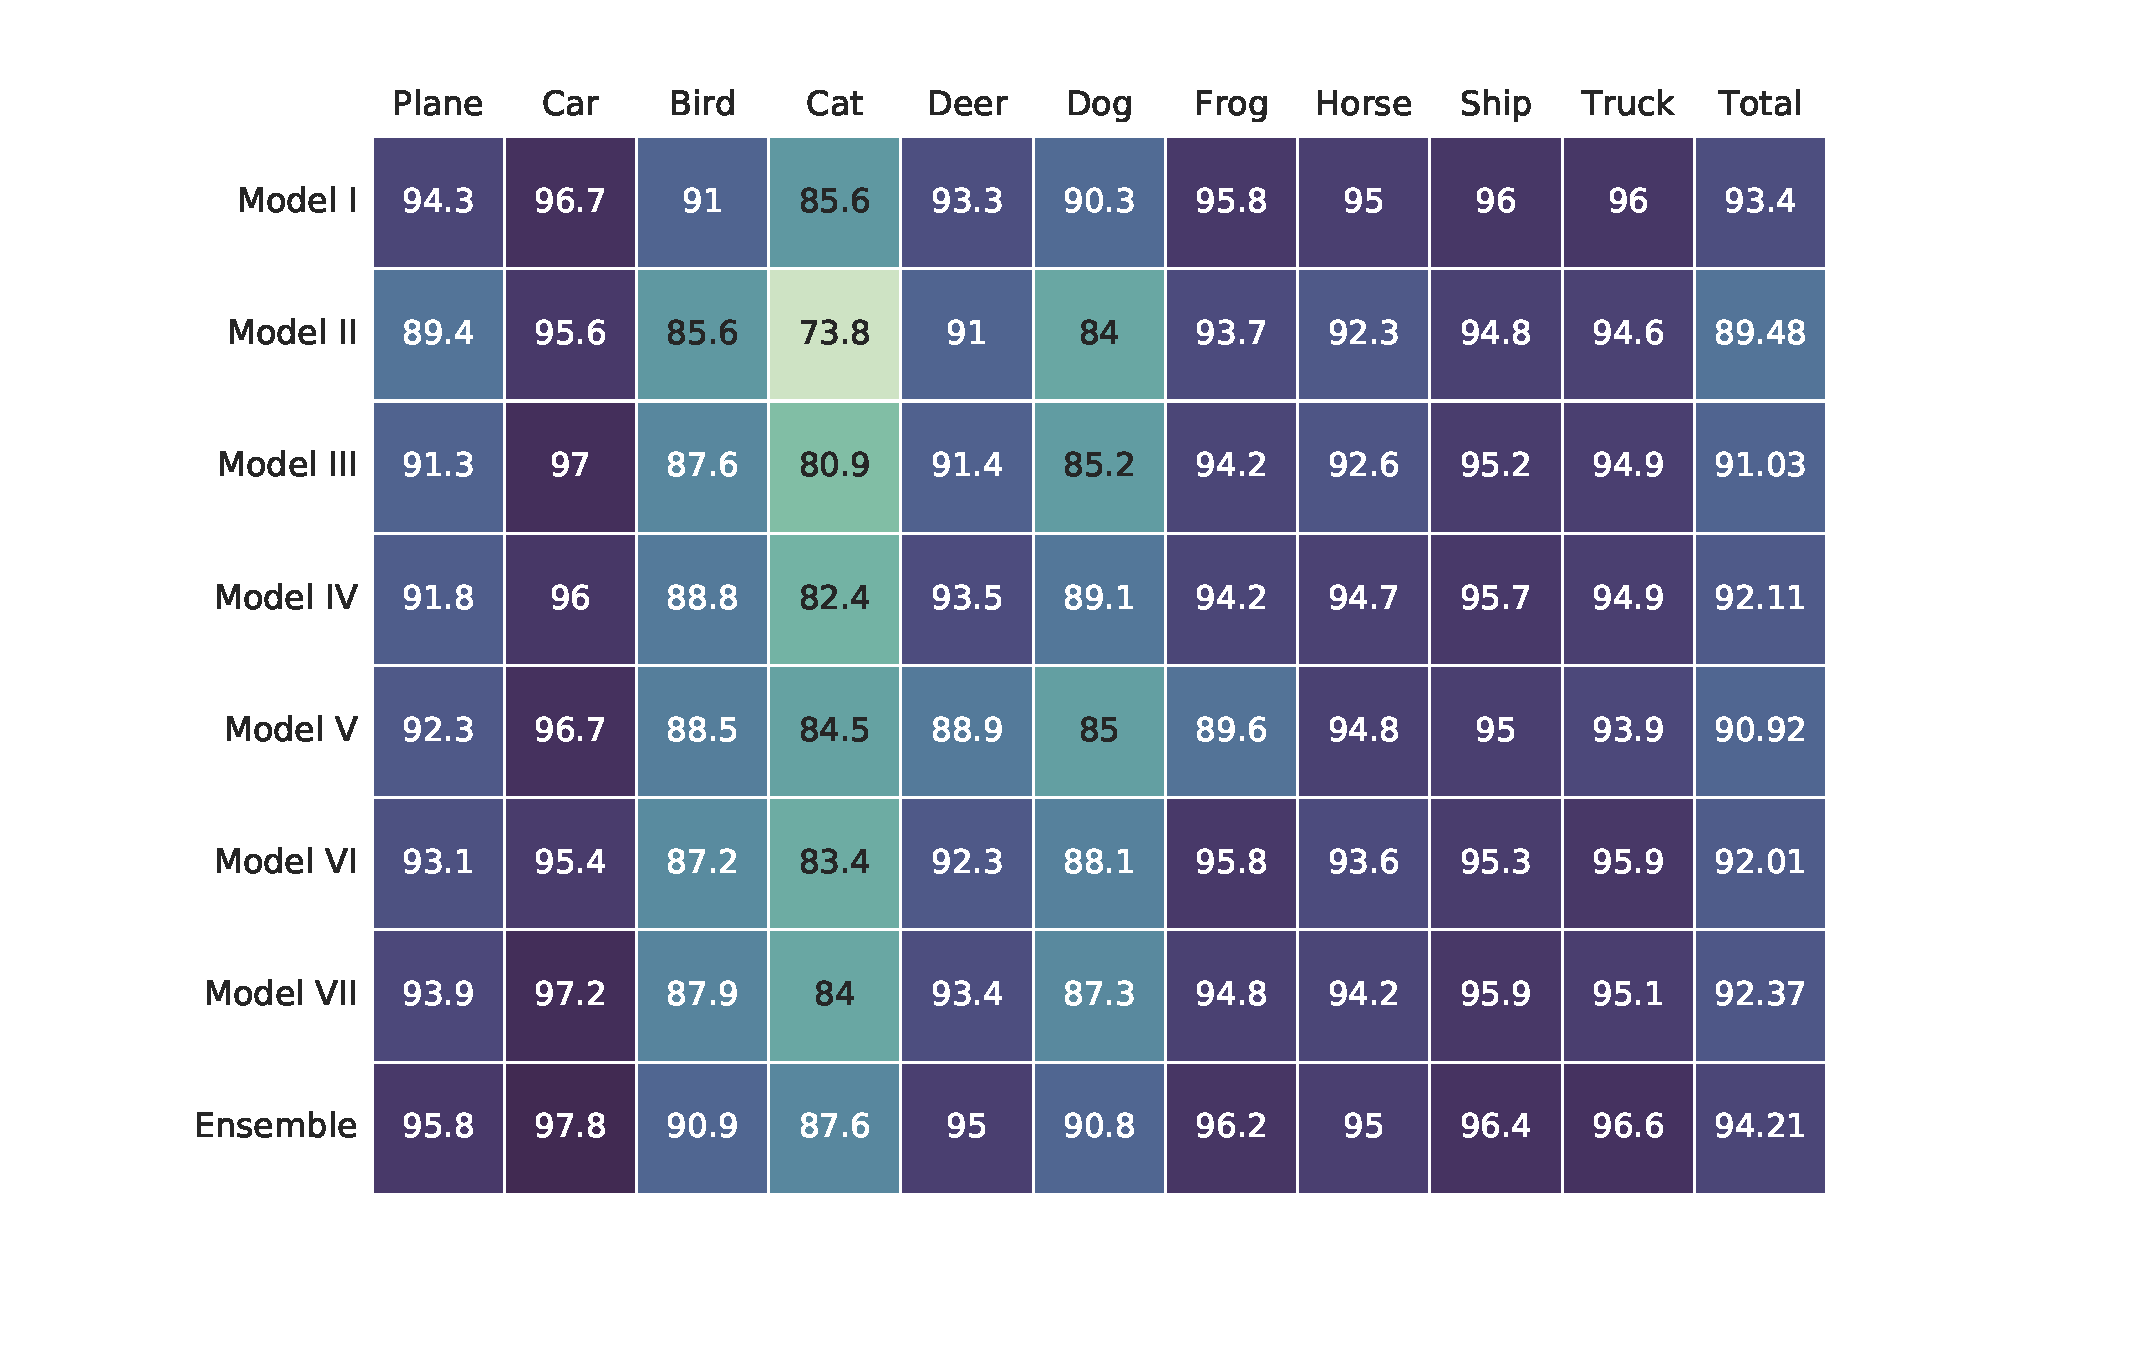
\includegraphics[width=\textwidth]{accuracy_table}
    \vspace*{-2cm}
    \caption{Точности распознавания по различным классам}
    \label{table-accuracy}
\end{figure}

\begin{figure}[H]
    \centering
    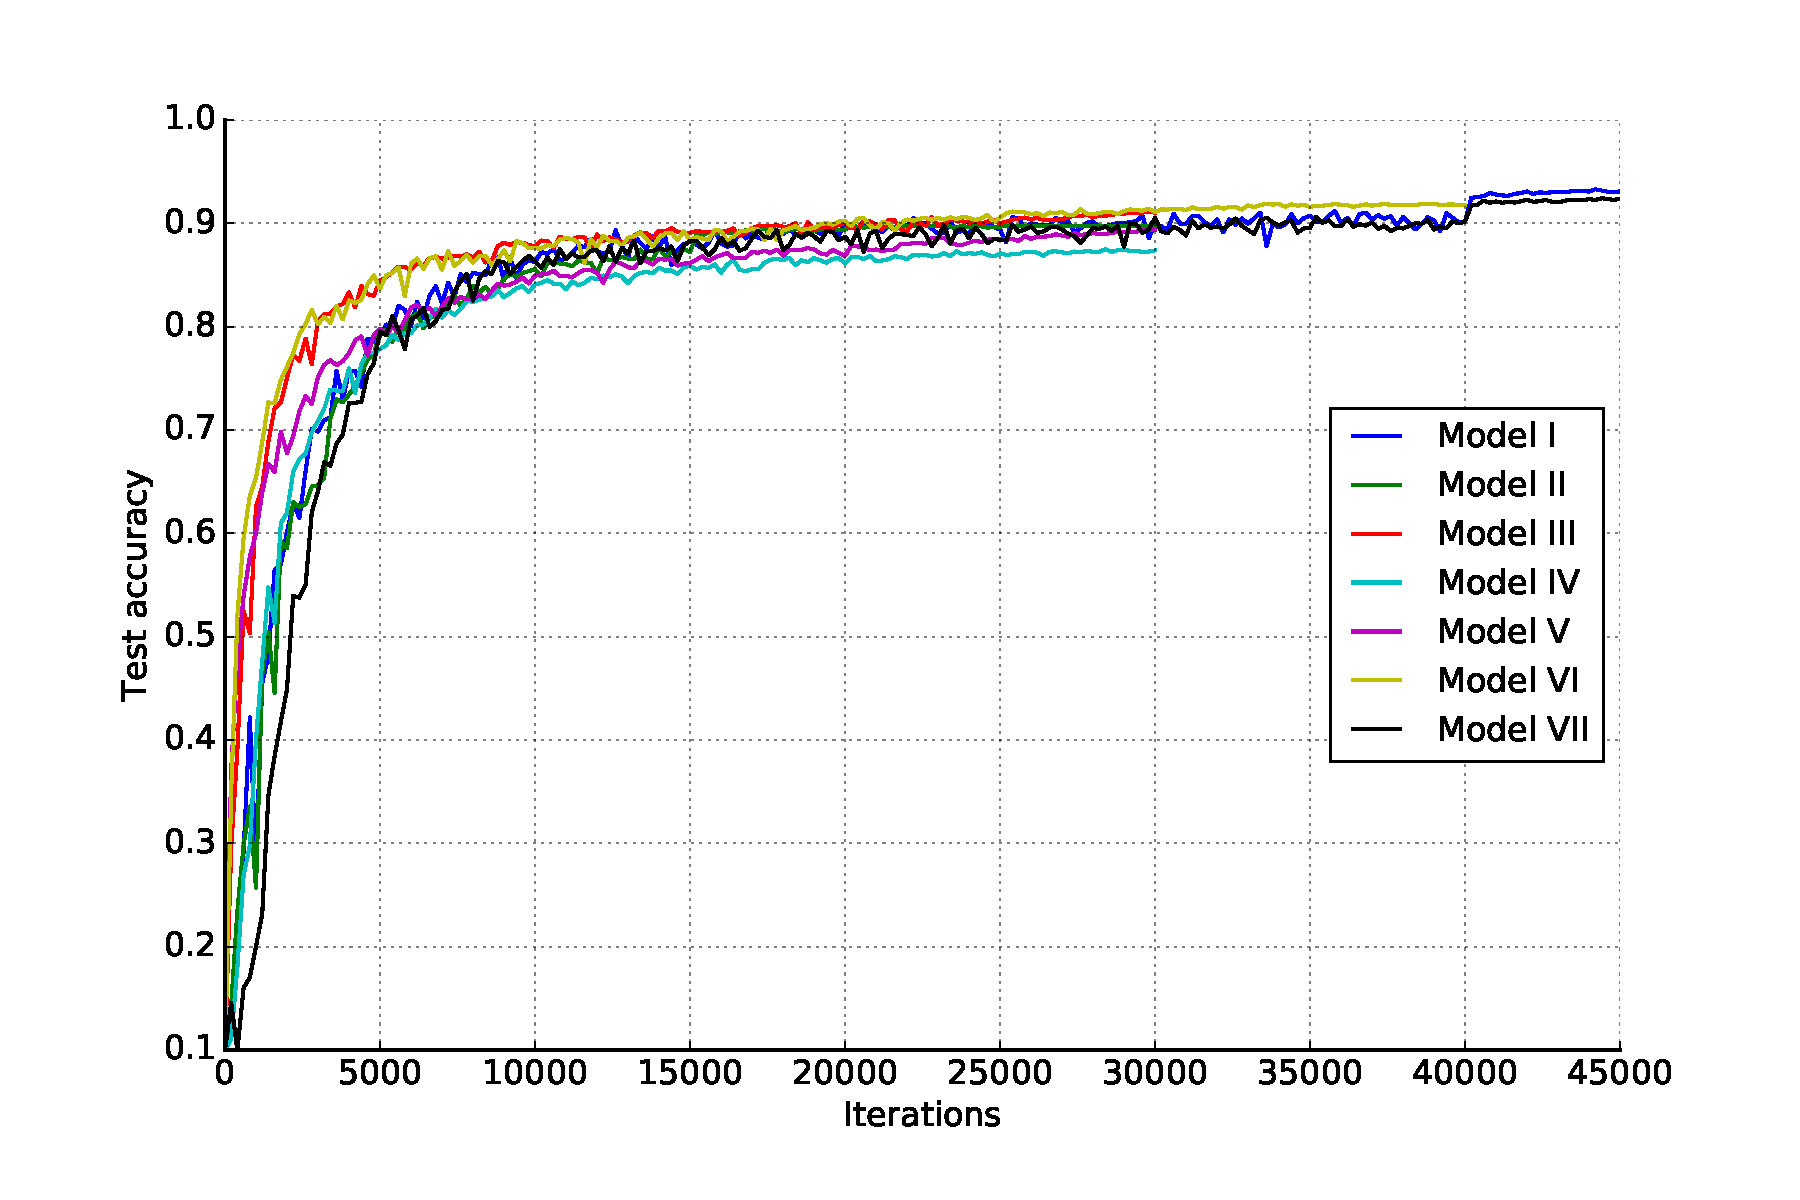
\includegraphics[width=\textwidth]{train_all}
    \vspace*{-1.3cm}
    \caption{Графики обучения моделей}
    \label{fig:train_all}
\end{figure}

\begin{figure}[H]
    \centering
    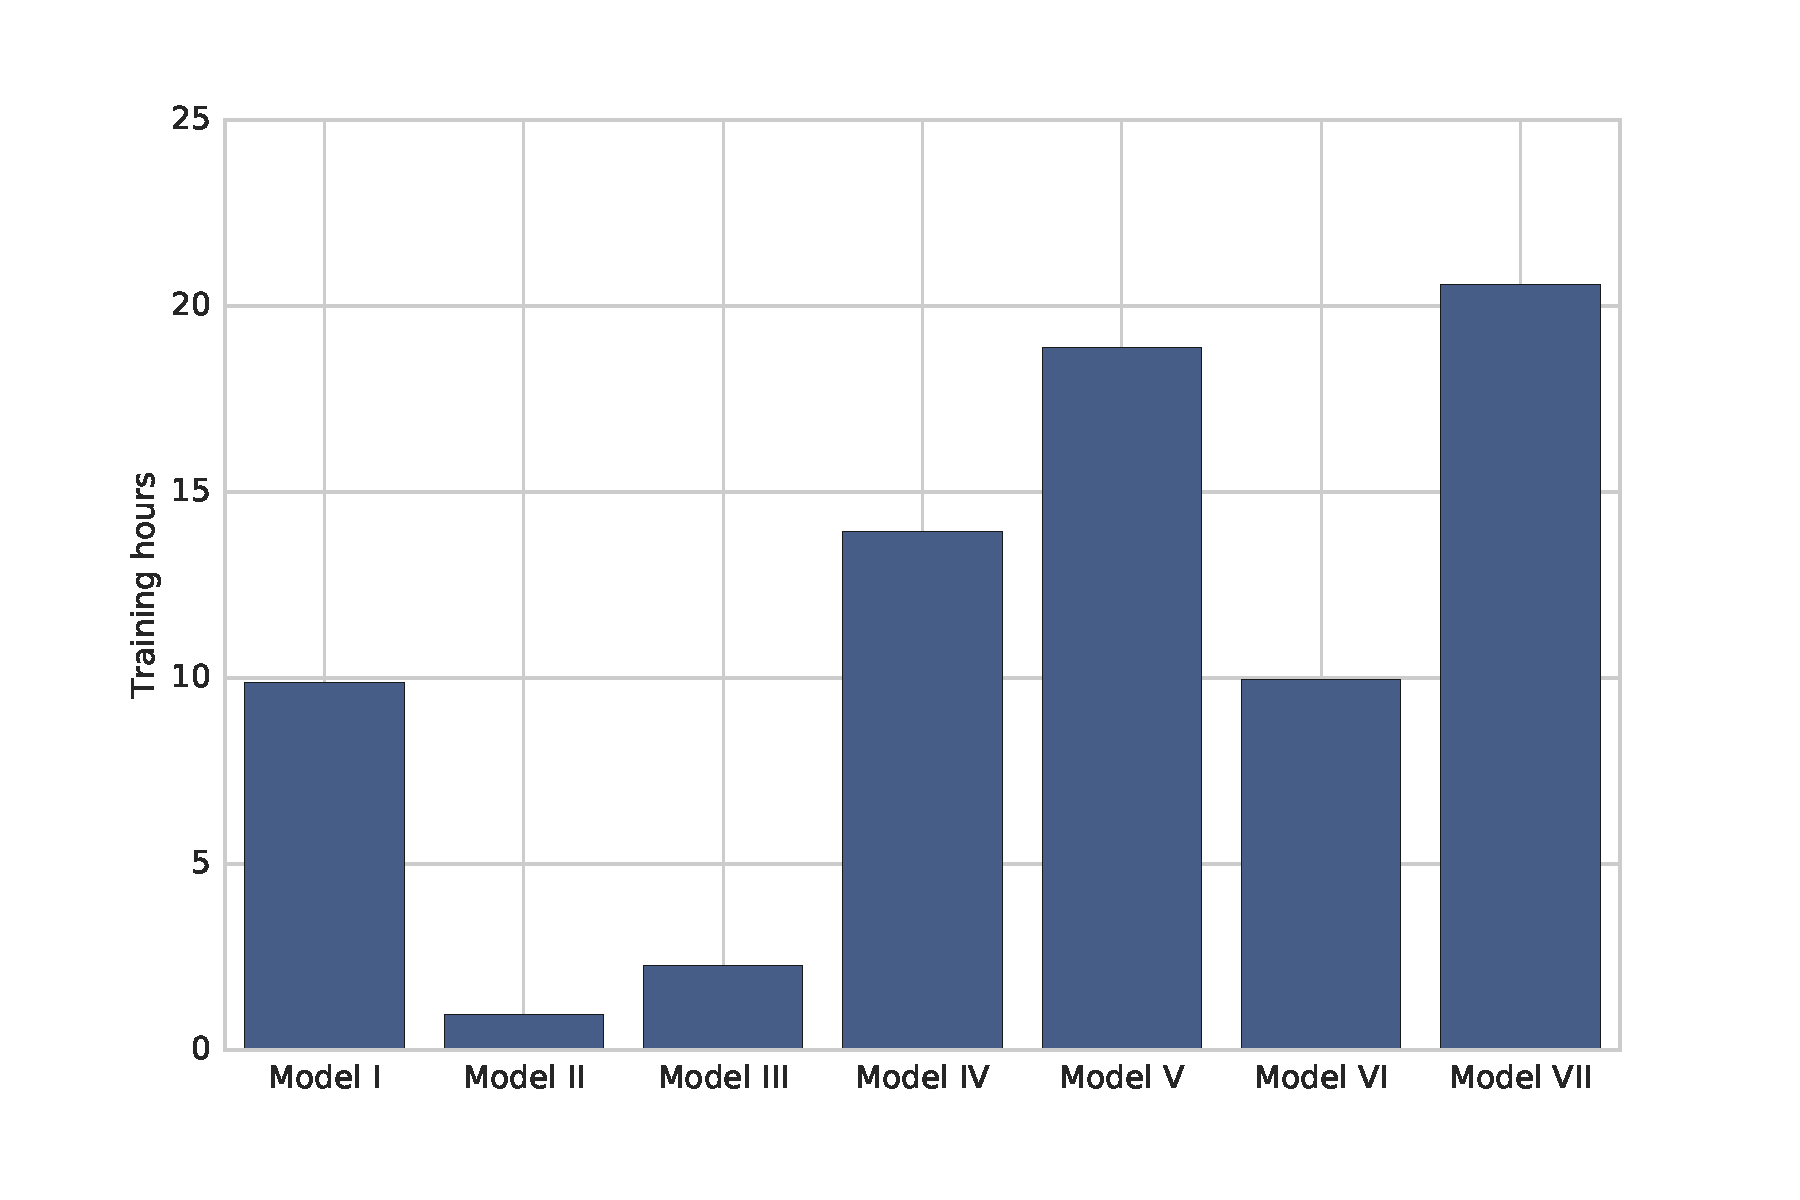
\includegraphics[width=0.9\textwidth]{time_consumption}
    \vspace*{-0.5cm}
    \caption{Время, затраченное моделями на обучение}
    \label{time_consumption}
\end{figure}
\clearpage

\lstinputlisting[language=Python, caption=Препроцессинг изображений]{CIFAR10_zca.py}
\lstinputlisting[language=Python, caption=Оценка модели и запись ответов в таблицу
                                          для дальнейшего построения ансамбля]{predict.py}
\lstinputlisting[language=Python, caption=Построение ансамбля из таблицы ответов нейронных сетей]{ensemble.py}